\documentclass[12pt, letterpaper]{article}

%-------Packages---------
\usepackage{amssymb,amsfonts}
\usepackage{mathptmx}
\usepackage{amsthm}
\usepackage{graphicx}
\usepackage[all,arc]{xy}
\usepackage{enumerate}
\usepackage{bbm}
\usepackage{dsfont}
\usepackage{mathrsfs}
\usepackage{tikz-cd}
\usepackage{setspace}
\usepackage{import}
\usepackage[utf8]{inputenc}
\usepackage{hyperref}
\usepackage{tikz}
\usepackage{float}
\usepackage[dvipsnames]{xcolor}
\usepackage[nocheck]{fancyhdr}
\usepackage[nointegrals]{wasysym}

\usepackage[left=1in,top=1in,right=1in,bottom=1in]{geometry}

\usepackage{mathtools}
\usepackage{setspace}
\usepackage{cleveref}
\usepackage{multicol}
\usepackage{mathpazo}
\usepackage{tcolorbox}
\tcbuselibrary{theorems,skins,breakable}
\usepackage{xparse}

\usepackage{algorithm}
\usepackage[noend]{algpseudocode}

\usepackage{xcolor, ifthen, tcolorbox}
\tcbuselibrary{theorems,skins,breakable}
% Theorem System
% The following environments are provided:
%   New Problem:        \begin{problem} ...
%   New Question Header:   \qh (then followed by subproblems)
%   Subproblem:     \begin{subproblem} ...
%   Problem Proof:  \begin{problemproof} ...
%   Proof:          \\begin{pf}{color} ...
%   Remark:         \rmk (sentence), \rmkb (block)

% Define custom colors
\definecolor{thmscol}{HTML}{F4565B} %For Problems
\definecolor{lemscol}{HTML}{FE844C} %For Lemmes
\definecolor{prpscol}{HTML}{00A7EF} %For proposition
\definecolor{corscol}{HTML}{23DAFF} %For corrolaries
\definecolor{rmkscol}{HTML}{6DEEC5} %For remarks
\definecolor{defscol}{HTML}{18C991} %For definitions
\definecolor{exmscol}{HTML}{7DB800} %For examples
\definecolor{clmscol}{HTML}{165c58} %For claims

%Change between dark(black)/light(white) mode
\newcommand{\colormode}{white}
\ifthenelse{\equal{\colormode}{white}}
      {\newcommand{\TextColor}{black}}
      {\newcommand{\TextColor}{white}}
\newcommand{\pbcolormain}{thmscol!80!\colormode}
\newcommand{\pbcolorsecond}{thmscol!38!\colormode}


% ============================
% Problem Counter
% ============================
\newcounter{subproblemcounter}
\newcounter{problemcounter}

\newcommand{\q}{
    \setcounter{subproblemcounter}{0}%
    \stepcounter{problemcounter} % Increment problem counter
    \color{\TextColor}Problem \arabic{problemcounter}: % Display the problem counter
}

\newcommand{\stepsub}{
    \stepcounter{subproblemcounter}%
    \color{\TextColor}(\alph{subproblemcounter})
}
% ============================
% Problem
% ============================
\newtcolorbox{pb}[1]{
  enhanced,
  frame hidden,
  titlerule=0mm,
  toptitle=1mm,
  bottomtitle=1mm,
  fonttitle=\bfseries\large,
  coltitle=black,
  colbacktitle=\pbcolormain,
  colback=\pbcolorsecond,
  title={\q #1},
  coltext=\TextColor
}

\newtcolorbox{spb}[1]{
  enhanced,
  frame hidden,
  titlerule=0mm,
  toptitle=1mm,
  bottomtitle=1mm,
  fonttitle=\bfseries\large,
  coltitle=black,
  colbacktitle=\pbcolormain,
  colback=\pbcolorsecond,
  title={\stepsub #1},
  coltext=\TextColor,
  attach boxed title to top left={xshift=3mm,yshift=-2mm},
  boxed title style={
    colback=\pbcolormain,
    colframe=\pbcolormain,
  }
}

\newtcolorbox{pbh}[1]{
    enhanced,
    frame hidden,
    titlerule=0mm,
    toptitle=1mm,
    bottomtitle=1mm,
    fonttitle=\bfseries\large,
    coltitle=black,
    colbacktitle=\pbcolormain,
    colback=\pbcolorsecond,
    title={\q #1},
    boxrule=0pt,
    interior hidden,
    attach boxed title to top left={xshift=3mm,yshift=-2mm},
    boxed title style={
        colback=\pbcolormain,
        colframe=\pbcolormain,
    }
}

\newenvironment{problem}[1]{%
  \newpage
  \begin{pb}{#1}
    }{
  \end{pb}
}

\newenvironment{subproblem}[1]{%
  \begin{spb}{#1}
    }{
  \end{spb}
}

\newenvironment{problemproof}{%
    \begin{pf}{\pbcolormain}
        }{
    \end{pf}
}

\newcommand{\qh}[1][]{
    \newpage
    \begin{pbh}{#1}\end{pbh} % Display the problem counter
}

% ============================
% Claim
% ============================

\newtcbtheorem[number within=problemcounter]{claim}{Claim}
{
    enhanced,
    frame hidden,
    titlerule=0mm,
    toptitle=1mm,
    bottomtitle=1mm,
    fonttitle=\bfseries\large,
    coltitle=black,
    colbacktitle=clmscol!50!\colormode,
    colback=clmscol!20!\colormode,
}{clm}

\NewDocumentCommand{\clm}{m+m}{
    \begin{claim*}{#1}{}
        #2
    \end{claim*}
}

\newenvironment{clmpf}{
	{\noindent{\it \textbf{Proof.}}
	\setlength{\parindent}{0pt}
	}
	\tcolorbox[blanker,breakable,left=5mm,parbox=false,
    before upper={\parindent15pt},
    after skip=10pt,
	borderline west={1mm}{0pt}{clmscol!50!\colormode}]
}{
    \textcolor{clmscol!50!\colormode}{\hbox{}\nobreak\hfill$\blacksquare$}
    \endtcolorbox
}

\NewDocumentCommand{\clmp}{m+m+m}{
    \begin{claim*}{#1}{}
        #2
    \end{claim*}

    \begin{clmpf}
        #3
    \end{clmpf}
}


% ============================
% Proof
% ============================

\newenvironment{pf}[1]{%
  \def\pfcolor{#1}% Store the color in a macro
  \noindent{\it \textbf{Proof.}}%
  \tcolorbox[blanker,breakable,left=5mm,parbox=false,%
    before upper={\parindent15pt},%
    after skip=10pt,%
    borderline west={1mm}{0pt}{\pfcolor},%
    coltext=\TextColor
  ]%
  \setlength{\parindent}{0pt}%
}{%
  \textcolor{\pfcolor}{\hbox{}\nobreak\hfill$\blacksquare$}%
  \endtcolorbox%
}

\newtcolorbox{solution}{
  blanker,
  breakable,
  left=5mm,
  parbox=false,%
  before upper={\parindent15pt},%
  after skip=10pt,%
  borderline west={1mm}{0pt}{\pbcolormain},%
  coltext=\TextColor
}


% ============================
% Remark
% ============================


\NewDocumentCommand{\rmk}{+m}{
    {\it \color{rmkscol!100!white}#1}
}

\newenvironment{remark}{
    \par
    \vspace{5pt}
    \begin{minipage}{\textwidth}
        {\par\noindent{\textbf{Remark.}}}
        \tcolorbox[blanker,breakable,left=5mm,
        before skip=10pt,after skip=10pt,
        borderline west={1mm}{0pt}{rmkscol!80!\colormode},
        coltext=\TextColor
        ]
}{
        \endtcolorbox
    \end{minipage}
    \vspace{5pt}
}

\NewDocumentCommand{\rmkb}{+m}{
    \begin{remark}
        #1
    \end{remark}
}


% Define a new command for problems
\renewcommand{\headrule}{\color{\TextColor}\hrulefill}
\newcommand{\C}{\mathbb{C}}
\newcommand{\R}{\mathbb{R}}
\newcommand{\Q}{\mathbb{Q}}
\newcommand{\Z}{\mathbb{Z}}
\newcommand{\N}{\mathbb{N}}
\renewcommand{\P}{\mathbb{P}}
\newcommand{\NP}{\mathsf{NP}}
\newcommand{\F}{\mathbb{F}}
\newcommand{\T}{\mathcal{T}}
\newcommand{\contr}{\Rightarrow \Leftarrow}
\newcommand{\s}{\(\,\)}
\renewcommand{\t}[1]{\text{#1}}
\newcommand{\ang}[1]{\left\langle #1 \right\rangle}
\newcommand{\coker}{\mathrm{coker}}

% Meta data
\setstretch{1.2}

\begin{document}
\color{\TextColor}
\pagecolor{\colormode}
\setlength{\parindent}{0pt}
\pagestyle{fancy}
\fancyhf{}
\fancyhead[LOE]{\color{\TextColor}\slshape{\textbf{Vincent Ferrara}}}
\fancyhead[ROE]{\color{\TextColor}\thepage}

\qh[Self assessment.]
\begin{solution}
    For problem 6 (a). I feel my solution is better because in the solution they have a for loop that loops $n$ times, but since $n$ is an integer it is size $\log(n)$ in terms of the input size, but they do a $O(n)$ operation, so if $n$ is really large it could be exponential in terms of the input. Thus, to fix this in my solution I checked if $n \geq |C|$, and if it was all you had to check if each $c_i \in C$ was less than the workload limit $k$.
\end{solution}

\begin{problem}{Uniform sampling with constant memory.}
    \vspace{-20pt}
    \begin{minipage}{\linewidth}
        \begin{algorithm}[H]
          \begin{algorithmic}[1]
            \Function{Uniform}{$a_1, \ldots, a_n$}
            % \State Store $a_1$ in memory
            \For{$i = 1, \ldots, n$}
              \State Overwrite the current memory with $a_i$ with probability $1/i$ 
              \State Otherwise, the memory stays unchanged (with probability $1 - 1/i$)
            \EndFor
            \State Output the item in the memory
            \EndFunction
          \end{algorithmic}    
        \end{algorithm}
      \end{minipage}
      \vspace{5pt}

      Prove that \textsc{Uniform} selects a uniformly random sample from the sequence $(a_1, \ldots, a_n)$. In other words, show that each element $a_i$ has an equal probability $1/n$ being in the memory after processing all items.
\end{problem}
\begin{problemproof}
    Let $\P(a_i)$ be the probability that $a_i$ is chosen at time $i$, and let $\P(\lnot a_j)$ be the probability that $a_j$ was not chosen at time $j$.

    Thus, $\P(a_i \t{ is the output})=\P(a_i \cap \lnot a_{i+1} \cap \dots \cap \lnot a_n)$ since all of these events are only dependent on time $t$. This implies that they are all indepdent of each other.

    Therefore,
    \begin{align*}
      \P(a_i \t{ is the output})&=\\
      &=\P(a_i \cap \lnot a_{i+1} \cap \dots \cap \lnot a_n)\\
      &=\P(a_1) \P(\lnot a_{i+1}) \dots \P(\lnot a_n)\\
      &=\dfrac{1}{i}\prod_{k = i+1}^n \left( 1- \dfrac{1}{j} \right)\\
      &=\dfrac{1}{i}\prod_{k = i+1}^n \left( \dfrac{j-1}{j} \right)=\dfrac{1}{i}\cdot\dfrac{i}{n}=\dfrac{1}{n}
    \end{align*}
    Therefore, each $a_i$ has an equal probability $1/n$ being the output.
\end{problemproof}

\begin{problem}{Recording record-breaking moments.}
  The \emph{Hall of Fame} has only \emph{one seat}, reserved for the current fastest time. Every time a record is broken, i.e., $t_i = \min\{t_1, \ldots, t_i\}$, the seat changes hands to the new record-holder. Lambda, who is responsible for updating the Hall of Fame, starts to wonder how often they will have to make these updates. 

For simplicity, you may assume all $t_i$'s are \emph{distinct} in this problem. 
\end{problem}

\begin{subproblem}{}
  Define an indicator random variable that is suitable for this problem. When defining an indicator random variable, be sure to:
    \begin{enumerate}
        \item clearly describe the event for which the variable equals 1 and 0 (you may write ``0 otherwise" to be concise), and
        \item derive the probability that the indicator random variable equals 1. 
    \end{enumerate}
\end{subproblem}
\begin{problemproof}
  Let $X_i$ be the random variable s.t. $X_i$ is 1 if $t_i$ is the minimum time of $\{t_1,\dots,t_i\}$ and 0 otherwise.

  $\P(X_i = 1)=\P(t_i=\min\{t_1,\dots,t_i\})=\dfrac{1}{i}$. Since all times are distinct and in a random order, every permutation of the times is equally likely thus since there is only one minimum in the first $i$ times this implies the probability is $1/i$.
\end{problemproof}

\begin{subproblem}{}
  Let $X$ be the number of record-breaking moments. Show that
    \[
        \mathbb{E}[X] = 1 + \frac{1}{2} + \ldots + \frac{1}{n}
    \]
\end{subproblem}
\begin{problemproof}
  Since $X$ is the number of record-breaking moments this happens exactly when $t_i$ is the minimum of all the previous times. Thus, this is exactly when $X_i=1$.

  Therefore, $X=X_1+\dots+X_n$.

  Thus, 
  
  $\mathbb{E}[X]=\mathbb{E}[X_1+\dots+X_n]=\mathbb{E}[X_1]+\dots+\mathbb{E}[X_n]=\P(X_1=1)+\dots+\P(X_n=1)=1+1/2+\dots+1/n$.
\end{problemproof}

\begin{problem}{Equi-satifiability.}
  In this problem, we define a clause to be in \emph{4-disjunctive-unique-form} (4DUF) if it has \emph{exactly 4 literals} involving \emph{4 distinct variables}, connected by disjunctions ($\lor$).

  Given a truth assignment, we say that 4DUF clause is \emph{equi-satisfied} if it contains \emph{exactly two} true literals and \emph{exactly two} false literals. 

  Now, consider a collection of $m$ 4DUF clauses $C = \{c_1, \ldots, c_m\}$. While a variable may appear in multiple clauses, no clause contains repeated variables. Let \textsc{Rand-Assign} be the same randomized algorithm as in lecture: assign random truth values (true or false) to the formula’s variables, uniformly and independently. That is, for each variable, assign it to be true or false each with $1/2$ probability, independently of all the others.
\end{problem}
\newcommand{\E}{\mathbb{E}}
\begin{subproblem}{}
  Show that \textsc{Rand-Assign} equi-satisfies a constant fraction $\rho \in [0,1]$ of the clauses of $C$ in expectation. Analyze and determine the exact value of $\rho$. 
\end{subproblem}
\begin{problemproof}
  Let $X$ be the number of equi-satisfied clauses of $C$.

  Let $X_i$ be $1$ if clause $c_i \in C$ is equi-satisfied and $0$ if not.

  Thus, $X=X_1+\dots+X_m$.

  Therefore, $\E[X]=\E[X_1]+\dots+\E[x_m]=\P(X_1=1)+\dots+\P(X_m=1)$.

  Since each variable in clause $c_i$ has a uniform probability of being true or false. This implies that the probability of being equi-satisfied is.

  Total outcomes: $2^4=16$ for all possible truth assignments

  equi-satisfied: The number of ways to choose exactly 2 out of the 4 to be true is $\binom{4}{2}=6$.

  Thus, $\P(X_i=1)=\dfrac{6}{16}=\dfrac{3}{8}$.

  Therefore, $\E[X]=m\dfrac{3}{8}$

  Thus, $\rho=\E[X]/|C|=3/8$
\end{problemproof}

\begin{subproblem}{}
  Using Markov's inequality, give a \textbf{lower bound} on the probability that \textsc{Rand-Assign} equi-satisfies at least $\rho/2$-fraction of the clauses.
\end{subproblem}
\begin{problemproof}
  Let $X$ be the number of equi-satisfied clauses of $C$. Let $Y=m-X$ which is the number of not equi-satisfied caluses.

  Thus by Markov's inequality, 
  
  $\P(Y \geq m(1-\rho/2)) \leq \dfrac{\E[Y]}{m(1-\rho/2)} = \dfrac{\E[m-X]}{m(1-\rho/2)}=\dfrac{m(1-\rho)}{m(1-\rho/2)}=\dfrac{1-\rho}{1-\rho/2}$.

  Also since if $X \leq \rho/2 \cdot m$ then
  \[Y=m-X > m-\rho/2 m = m(1-\rho/2) \implies \P(X < \rho/2 m) \leq \P(Y \geq m(1-\rho/2))\]

  Thus, $\P(X < \rho/2 \cdot m) \leq \dfrac{1-\rho}{1-\rho/2}$

  Since $\P(X < \rho/2\cdot m)=1-\P(X \geq \rho/2 \cdot m)$, this implies that $\P(X \geq \rho/2 \cdot m) \geq 1-\dfrac{1-\rho}{1-\rho/2}$.

  Since $\rho=3/8$. This implies that $\P(X \geq 3/16 \cdot m) \geq 1-\dfrac{10}{13}=\dfrac{3}{13}$
\end{problemproof}

\begin{problem}{}
  Let~$S$ be a set of~$n$ orderable elements, which are distinct without loss of generality.
  We say that $a\in S$ has \emph{rank} $\t{rank}(a)=k$ if~$a$ is the $k$th smallest element in $S$.
  Given input~$S$, the goal is to find a \emph{near median} of~$S$, which is an element having rank between $2n/5+1$ and $3n/5$ (inclusive).
  For simplicity, \emph{we assume that~$n$ is divisible by 5} (because we can ``pad'' the set with up to four extra elements).
\end{problem}

\begin{subproblem}{}
  Consider the simplest randomized algorithm: output a uniformly random element $a \in S$.
    
    Prove that this algorithm outputs a near median of~$S$ with probability at least $1/5$.
\end{subproblem}
\begin{problemproof}
  Since there are $\dfrac{3n}{5}-\dfrac{2n}{5}-1+1=\dfrac{n}{5}$ elements between $[2n/5+1,3n/5]$.

  This implies there are $n/5$ near medians.

  Therefore, since each element has a uniform chance of being picked this implies that there is a $(n/5)/(n)=1/5$ probability of $a$ being a near median.
\end{problemproof}

\begin{subproblem}{}
  Briefly describe an $O(n)$-time algorithm that, given~$S$ and an element $a \in S$, determines whether~$a$ is a near median.
\end{subproblem}
\begin{problemproof}
  Just traverse the set $S$ and count the number of elements s.t. $b < a$ for $b \in S$ call this number $k$. Thus, $\t{rank}(a)=k+1$ since $k$ elements are smaller than $a$.

  Now if $k+1 \in [2n/5+1,3n/5]$ then $a$ is near median otherwise it is not.

  This is $O(n)$ since we just traverse the array which has $n$ things in it, and the rest are $O(1)$ operations.

  This is correct since we defined near median to be if the rank is in the set $[2n/5+1,3n/5]$.
\end{problemproof}

\begin{subproblem}{}
  Give an $O(n)$-time randomized algorithm that, on input~$S$, outputs a near median with probability at least 99\%.
\end{subproblem}
\begin{problemproof}
  Since the probability of picking a near median is $n/5$ this implies the probability of not picking a near meadian is $(4/5)$. Thus, if we randomly pick $k$ times we would have a probability of $(4/5)^k$ of not getting a near median once.

  Thus, for the failure to be at most 1\% we get that $(4/5)^k \leq 0.01 \implies k \log(4/5) \leq \log(0.01) \implies k \geq 20.7$ Thus, let $k=21$.

  Thus for $i=1 \t{ to } 21$ pick an element $a$ from $S$ then run the algorithm from $b$ on it to check if it is near median. If it is then return $a$ and halt.

  If we found no near medians for all of the 21 iterations then just output the most recent pick.

  Runtime:

  This is $O(21n)=O(n)$.

  Correctness:

  Since we have show that the chance of not picking a near median in 21 trials is less than 1\%. This implies our algorithm with output a near median with probability of at least $99\%$.
\end{problemproof}

\begin{problem}{Random binary search trees.}
  For a random binary search tree on $1, \ldots, n$, prove that the expected depth of the node with any particular value is $O(\log n)$.
  In other words, for any particular value in a random binary search tree, searching for it takes $O(\log n)$ time.
\end{problem}
\begin{problemproof}
  Let $v \in \{1,\dots,n\}$.

  For each $j \neq v$ $X_j=1$ if $j$ is an ancestor of $v$, and 0 otherwise.

  Thus, for $X$ being the depth of $v$ is equal to $X=\sum_{j \neq v} X_j$.

  Therefore, $\E[X]=\sum_{j \neq v}\E[X_j]=\sum_{j \neq v} \P(X_j = 1)$.

  If $j < v$. For $j$ to be an ancestor of $v$, it must be the first element chosen among all the elements in the interval $\{j,\dots,v\}$. Since if $j$ is picked first then $j$ becomes the root to all elements in $\{j+1,\dots,v\}$.

  If $j$ is not picked first and lets say $k \in \{j+1,\dots,v-1\}$ is then this would mean that $k$ would become the root, 
  and we would split the tree s.t. $\{j,\dots,k-1\}$ is in the left subtree and $\{k+1,\dots,v\}$ are in the right subtree. Thus, $j$ would not be an ancestor of $v$.

  Thus, the probability of picking $j$ first out of this set is $\dfrac{1}{v-j+1}$ since we pick each element with uniform probability.

  Thus, using the similar argument for $j > v$ we get $\dfrac{1}{j-v+1}$ probability of $j$ being an ancestor.

  Therefore,
  \begin{align*}
    \E[X]&=\sum_{j=1}^{v-1}\dfrac{1}{v-j+1} + \sum_{j=v+1}^n \dfrac{1}{j-v+1}\\
         &\leq \sum_{k=1}^{v-1} 1/k + \sum_{k=1}^n 1/n\\
         &\leq 2\ln(n)+2 = O(\log n)
  \end{align*}

  Therefore, the expected depth of $v \in \{1,\dots,n\}$ is $O(\log n)$
\end{problemproof}

\begin{problem}{Randomized vertex cover.}
  In this problem, we will consider randomized algorithms for approximating vertex-cover problems. Recall that the ``double cover'' algorithm \emph{deterministically} gives a 2-approximation to the minimum vertex cover problem, but in this problem you will show that a randomized approach is more versatile.
\end{problem}

\begin{subproblem}{}
  Consider a probability experiment with set $S$ with $k$ distinct items. In each round: 
  \begin{itemize}
      \item With probability \textbf{at least} $p$ (where $p \in (0,1]$), one \emph{new} item (not previously chosen) is selected. 
      \item Otherwise, no item is selected on that round. 
      \item The experiment ends when all $k$ items are selected. 
  \end{itemize}

  Let $R$ be a random variable denoting the number of rounds until the experiment ends. Prove that
  \[
    \E[R] \leq \frac{k}{p} 
  \]

\end{subproblem}
\begin{problemproof}
  For each $i=1,\dots,k$, define $R_i$ as the number of rounds needed to select the $i$-th new item after $i-1$ items have been choosen.

  Since the experiment finishes when all $k$ items are chosen, the total number of rounds $R$ to complete the experiment can be expressed as
  \[R=R_1+\dots+R_k\]

  Since $R_i$ is the number of rounds until one success of picking an item. It is a geometric random variable. Also, since the probability of picking one item is greater than or equal to $p$ this implies that $\P(R_1=i) \leq (1-p)^{i-1}p$.

  Also since the probability of picking an item after picking $j$ items or picking $i$ items this implies that the distributions are the same. Therefore, $\P[R_i=c]=\P[R_j=c] \implies \E[R_i]=\E[R_j]$ for all $i,j$.

  Therefore,

  \begin{align*}
    \E[R]=\sum_{i=1}^k \E[R_i]&=k\E[R_1]\\
    &=k\sum_{i=1}^\infty i \P[R_1=i]\\
    &\leq k\sum_{i=1}^\infty i(1-p)^{i-1}p\\
    &= \frac{kp}{(1-1+p)^2}=\frac{k}{p}
  \end{align*}
\end{problemproof}

\begin{subproblem}{}
  Consider the following algorithm 

    \begin{minipage}{\linewidth}
      \begin{algorithm}[H]
        \begin{algorithmic}[1]
          \Function{RandomSingleCover}{$G = (V,E)$}
          \State{$C \gets \emptyset$}
          \While{there is some edge $e = (u,v)$ that is not covered by~$C$}
          \State{Add exactly one of $u$ or $v$ to $C$, each with probability $1/2$}
          \EndWhile
          \State{\Return{$C$}}
          \EndFunction
        \end{algorithmic}    
      \end{algorithm}
    \end{minipage}

    Prove that \textsc{RandomSingleCover} outputs a 2-approximation, in expectation, for the minimum vertex cover problem. In other words, show that
  \[
    \E[|C|] \leq 2 \cdot |C^*|
  \]
  where $C^* = \{v_{1}, \ldots, v_{k}\}$ is some minimum vertex cover in the input graph.
\end{subproblem}
\begin{problemproof} 
  Let 
  \[
  S_{\text{chosen}} \subseteq C^*
  \]
  denote the set of vertices from the minimum vertex cover \(C^*\) that have been “hit” (i.e., chosen by the probability experiment) up to the current iteration. We show by induction that after every iteration,  
  \[
  S_{\text{chosen}} \subseteq C,
  \]
  where \(C\) is the set of vertices chosen by the algorithm.

  Induction:

  Base Case:

  Before any iteration, the algorithm initializes \( C = \varnothing \). Correspondingly, no vertex from \(C^*\) has been chosen by the experiment yet, so \( S_{\text{chosen}} = \varnothing \). Clearly, \(\varnothing \subseteq \varnothing\).

  Inductive Step:

  Assume that after some iteration the invariant holds, that is, \(S_{\text{chosen}} \subseteq C\). Now consider an iteration where the algorithm processes an edge \(e = (u,v)\) that is currently uncovered by \(C\). Because \(C\) already contains all previously chosen vertices in \(C^*\) (by the inductive hypothesis), neither \(u\) nor \(v\) is in \(S_{\text{chosen}}\). Since \(C^*\) is a vertex cover, it must cover every edge in the graph, so the edge \(e\) must satisfy 
  \[
  \{u,v\} \cap (C^* \setminus S_{\text{chosen}}) \neq \varnothing.
  \]
  Upon processing \(e\), the algorithm adds one of its endpoints with probability \(1/2\). Hence, with probability at least \(1/2\) (or even higher if both endpoints belong to \(C^* \setminus S_{\text{chosen}}\)), the chosen vertex belongs to \(C^*\setminus S_{\text{chosen}}\). In that case, it is immediately included in \(C\), and we can consider it as being added to \(S_{\text{chosen}}\) with the ongoing experiment. If we did not pick the vertex that was in $C^*$ then this is associated to in the experiment when we do not choose an item, so $S_{\t{chosen}}$ remains the same thus \(C^*\setminus S_{\text{chosen}}\).
 
  Next, we show that the algorithm terminates by the time the probability experiment terminates.

  Suppose, for contradiction, that the probability experiment has terminated that is, but the algorithm has not yet terminated. Then there exists at least one edge \(e=(u,v)\) that remains uncovered by \(C\).

  However, since we have maintained the invariant \(S_{\text{chosen}} \subseteq C\) and \(S_{\text{chosen}} = C^*\), it follows that every vertex in \(C^*\) is also in \(C\). Because \(C^*\) is a vertex cover, every edge in the graph must be covered by some vertex in \(C^*\). Therefore, the edge \(e\) must be covered by \(C\), which is a contradiction. This implies that if the experiment terminates, the algorithm must also have terminated. In other words, the algorithm halts no later than the experiment does.

  Each iteration of the algorithm corresponds exactly to one round of the probability experiment, with one vertex being added to \(C\) per iteration. Let \(R\) denote the total number of rounds (or iterations) performed by the algorithm. From the analysis in part (a) of the problem, we know that if an experiment selects one new vertex from \(C^*\) in each round with a success probability of at least \(1/2\), then the expected number of rounds needed to select all \(|C^*|\) vertices is at most
  \[
  \mathbb{E}[R]=\mathbb{E}[|C|] \le \frac{k}{\frac{1}{2}} = 2k.
  \]
  Thus, the algorithm is a 2-approximation in expectation for the minimum vertex cover problem.
\end{problemproof}

\begin{subproblem}{}
  For each of the following algorithms, show that it can yield an \emph{arbitrarily large} approximation ratio for this problem, by describing an explicit graph and showing how the (expected) weight of the algorithm's output cover can be very large relative to the optimal weight.
    \begin{enumerate}[(i)]
    \item The double-cover algorithm from lecture.
    \item The \textsc{RandomSingleCover} algorithm from \cref{Rand-VC-Single}.
    \item The following greedy algorithm:
    \end{enumerate}
    \begin{minipage}{\linewidth}
      \begin{algorithm}[H]
        \begin{algorithmic}[1]
          \Function{Greedy}{$G = (V,E,w)$}          
          \State{$S \gets \emptyset$}
          \While{$G$ has an edge}
          \State{Remove all isolated vertices of $G$}
          \State{Add a lowest-weight vertex in $G$ to $S$ and remove all its incident edges}
          \EndWhile
          \State{\Return{$S$}}
          \EndFunction
        \end{algorithmic}
      \end{algorithm}
    \end{minipage}
\end{subproblem}
\begin{problemproof}
  Let $X$ be the weight of the algorithm's vertex cover.

  Fix $N > 1 \in \N$.

  Consider the graphs
  \begin{center}
    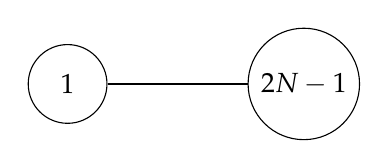
\begin{tikzpicture}
      % Define the vertices
      \node[draw, circle, minimum size=1cm] (A) at (0,0) {$1$};
      \node[draw, circle, minimum size=1cm] (B) at (3,0) {$2N-1$};
    
      % Draw an edge between the vertices
      \draw (A) -- (B);
    \end{tikzpicture}
    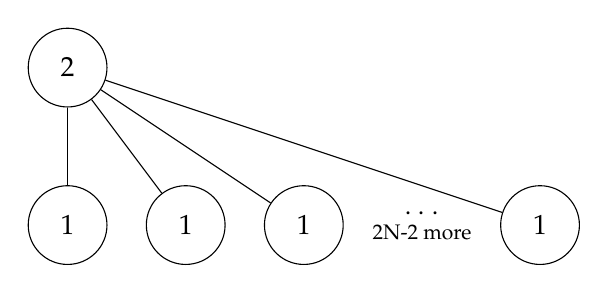
\begin{tikzpicture}
      % Top vertex (upper part of the bipartite graph) labeled "2"
      \node[draw, circle, minimum size=1cm] (Top) at (0,2) {2};
      
      % Bottom part: two explicit vertices on the left and right,
      % with an ellipsis in the middle to indicate more vertices.
      \node[draw, circle, minimum size=1cm] (B1) at (0,0) {1};
      \node[draw, circle, minimum size=1cm] (B2) at (1.5,0) {1};
      \node[draw, circle, minimum size=1cm] (B3) at (3,0) {1};
      \node at (4.5,0) {$\underset{\t{2N-2 more}}{\cdots}$};
      \node[draw, circle, minimum size=1cm] (B4) at (6,0) {1};
      
      % Connect the top vertex to the explicit bottom vertices
      \draw (Top) -- (B1);
      \draw (Top) -- (B2);
      \draw (Top) -- (B3);
      \draw (Top) -- (B4);
    \end{tikzpicture}
    
  \end{center}

  The optimal vertex cover for the graph to the left is to just pick the vertex with weight 1.

  The optimal vertex cover for the graph to the right is to just pick the vertex with weight 2.

  \begin{enumerate}[(i)]
    \item Look at the graph with two vertices. Since there is only one edge and the algorithm always picks both vertices this implies that 
    $\E[X]=2N \leq 2N\textsc{OPT}=2N$

    \item Look at the graph with two vertices. Since there is only one edge and each vertex has an equal chance of being picked this implies that $\E[X]=(1/2)1+(1/2)(2N-1)=N \leq N \textsc{OPT}=N$
    
    \item Look at the graph with $2N+1$ vertices. By defintion of the algorithm it will add all the ones to our cover first, but then since all of the ones are connected to $2$ it will disconnect 2 so we will be done. THus, we will have a total eight of $2N$. Thus, $\E[X]=2N \leq N \text{OPT} = 2N$.
  \end{enumerate}

  Therefore, for all of these algorithms there is a graph that will yield an arbitrarily large approximation ratio.
\end{problemproof}

\begin{subproblem}{}
  
\end{subproblem}
\begin{problemproof}
  Consider the following algorithm let $w(v)$ be the weight of vertex $v$.

    \begin{minipage}{\linewidth}
      \begin{algorithm}[H]
        \begin{algorithmic}[1]
          \Function{RandomWeightCover}{$G = (V,E)$}
          \State{$C \gets \emptyset$}
          \While{there is some edge $e = (u,v)$ that is not covered by~$C$}
          \State{Add exactly one of the vertices, and pick $u$ with probability $\dfrac{w(v)}{w(v)+w(u)}$}
          \EndWhile
          \State{\Return{Sum of $C$}}
          \EndFunction
        \end{algorithmic}    
      \end{algorithm}
    \end{minipage}

    Let $C^*$ be an optimal vertex cover and let $a \in C^*$. First partition $E$ s.t. each edge is assigned to a vertex in $C^*$. We can do this since $C^*$ is a vertex cover, so every edge is connected. We want to do this because we only want to look at each edge once, and it is easier to look locally at vertices in $C^*$.
    
    Consider $P(a) \subset E$ all of the edges that are assigned to $a$. For each $e \in P(a)$ since our algorithm's output is a vertex cover $C$ this means that at most one vertex of $e$ was added to $C$. Therefore, let $V_a$ be the set of vertices added by the algorithm that are connected to $P(a)$.

    Induction: We will induct on the size of $P(a)$, and show that $E[\sum_{v \in V_a}w(v)] \leq 2w(a)$.

    Base Case: $k=0$

    Then this implies that either $V_a=\emptyset$. Thus, $E[\sum_{v \in V_a}w(v)]=0 \leq 2w(a)$.

    Inductive Step: Assume that for all $k \leq n$: Consider $k=n+1$.

    First, consider $v' \in V_a$. Thus, $(a,v') \in P(a)$, and
    
    \begin{align*}
      E[\sum_{v \in V_a}w(v)]&=\P(v' \t{ being picked})[w(v')+E[\sum_{v \in V_a \setminus\{v'\}}w(v)]]+\P(a \t{ being picked})w(a)
      \intertext{The reason why this is correct because in case 1 our algorithm picked v', and thus we have to also account for the rest of the edges in $P(a)$, but in the other case if we pick $a$ then we are done since we will now cover all of $P(a)$}
      &=\frac{w(a)}{w(a)+w(v')}[w(v')+E[\sum_{v \in V_a \setminus\{v'\}}w(v)]]+\frac{w(v')}{w(a)+w(v')}w(a)
      \intertext{Thus, by induction hypothesis since $V_a \setminus {v'}$ is size $n$ we get that}
      &\leq 2\frac{w(a)w(v')}{w(a)+w(v')}+ 2\frac{w(a)^2}{w(a)+w(v')}=2w(a)\frac{w(v')+w(a)}{w(a)+w(v')}=2w(a)\\
    \end{align*}

    Therefore, $E[\sum_{v \in C}w(v)]=E[\sum_{a \in C^*} \sum_{v \in V_a}w(v)]$

    The reason this is true is because the $V_a$'s form a partition because we assign each edge in the graph uniquely to a vertex in the optimal vertex cover \(C^*\), ensuring that every edge is covered exactly once. Specifically, for each vertex \(a \in C^*\) we define \(P(a)\) as the set of edges assigned to \(a\). Since every edge is incident to at least one vertex in \(C^*\), and we assign it to just one vertex, the \(P(a)\)'s are disjoint. Then, for each \(a\), the set \(V_a\) is defined as all vertices chosen by the algorithm that are incident to at least one edge in \(P(a)\). As a result, every vertex added by the algorithm is uniquely associated with one of the \(P(a)\)'s ensuring that each such vertex is counted in exactly one \(V_a\). Therefore, the collection \(\{V_a : a \in C^*\}\) forms a partition of the set of vertices selected by the algorithm.

    Thus, $E[\sum_{a \in C^*} \sum_{v \in V_a}w(v)]=\sum_{a \in C^*}E[\sum_{v \in V_a}w(v)] \leq \sum_{a \in C^*}2w(a) = 2 \textsc{OPT}$.
\end{problemproof}
\end{document}